% \documentclass{standalone}
% \usepackage{currfile,hyperxmp}

% \input{../tikz_header.tex}

% \begin{document}



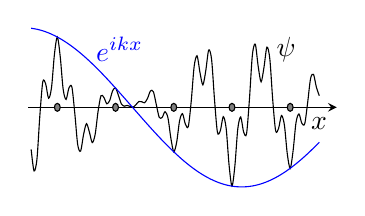
\begin{tikzpicture}
%\useasboundingbox (-1.3,-1.2) rectangle (10.2,4.7);
%\draw (-1,-1) rectangle (4,4);

    \begin{axis}[ %xlabel={Temperatur $T$  (K)}, ylabel={$C$ (mJ/mol K)}, 
         width=55mm, height=40mm, 
        %xmode=log, ymode=log,
         xmin = 0.5,xmax=5.8,
         % ymin = 0, ymax=7.5,
         axis x line=middle,
         axis y line=none,
         xtick = \empty, xticklabel = \empty,
         % xmax= 2e5, unbounded coords=jump, ymin=0, ymax = 4
        % label style={font=\tiny},
        % tick label style={font=\tiny}  
    ]


    \addplot[no marks, color=black, domain = 0.55:5.5,samples=100,smooth] {( cos(360 * x) + 0.5 * cos(360 * x * 4))/1.5 * cos(360* x / 7.5 - 20)};
    \addplot[no marks, color=blue, domain = 0.55:5.5,samples=50,smooth] {cos(360* x / 7.5 - 20) };

    \pgfplotsinvokeforeach{1,...,5}{
        \draw [fill=gray] (#1,0) circle (0.05);
    }
    
    \node[anchor= north east]  at (axis cs:5.8,0){ $x$};
    \node[anchor= north west, blue]  at (axis cs:1.5,1){ $e^{i k x}$};
    \node[anchor= north west]  at (axis cs:4.6,1){ $\psi$};
  

   % \addplot[no marks, color=black,dashed, domain = 0:6] {11 / 6^3 * x^3};
   % \addplot[no marks, color=blue, domain = 0:6] {11 / 6^3 * x^3 + 5.5 / 7 * x};
	
   % \addplot[no marks, color=blue, domain =30:100] {100 / x};

   % \addplot[no marks, color=red, domain = 70:500] {x^1 * exp(670/x) * 1e-8} ;


    %  \node[anchor=north east]  at (axis cs:30,4){x20};
	% \draw [dashed] (axis cs:30,0) -- (axis cs: 30,4);
	
	%      \node[anchor= west]  at (axis cs:0.4,3){ $\epsilon'$};
    %  \node[anchor= west]  at (axis cs:3,1){ $\epsilon''$};
   
    %  \node[anchor= west]  at (axis cs:150,3){ $\epsilon'$};
    %  \node[anchor= west]  at (axis cs:200,0.6){ $\epsilon''$};

    \end{axis}
\end{tikzpicture}

%\end{document}